\section{Lezione 2016-10-13}
\subsection{TODO}
% Insert what you need. Any row is associated with the improvment or mistake
% arise. In the first column you can insert what you should resolve or change,
% instead in the second column you may put the section where to apply some
% modification.
\begin{table}[ht]
\begin{center}
\begin{tabular}{|p{\textwidth}|c|}
\hline
\multicolumn{1}{|c|}{\textbf{Miglioramento}} & \textbf{Sezione} \\ \hline
Capire meglio come creare il primo stato del DFA nel $LR(k)$ parsing &
\ref{sec:risoluzione_conflitti} \\ \hline
Comprendere cos'\`e un \textit{viable prefix} &
\ref{sec:viable_prefix_and_valid_items} \\ \hline
Il punto 8 da automa a tabella del parsing $LR$ non \`e chiaro &
\ref{sec:step_parsing_table_construction_LR0} \
\ref{sec:step_parsing_table_construction_LR1} \\ \hline
Merge del $LALR$ non chiaro cosa si intende con la prima parte comune e l'
esempio non chiarisce & \ref{sec:parse_lalr} \
\href{http://www.di.unipi.it/~andrea/Didattica/PLP-16/SLIDES/PLP-2016-08.pdf}{
Slide n.47-49
} \\ \hline
\end{tabular}
\end{center}
\caption{Tabella miglioramenti}
\label{tab:tab_todo}
\end{table}

\subsection{Shift-Reduce Parsing}
Lo \textit{Shift-Reduce Parsing} \`e un tipo di parsing \textbf{bottom-up} dove
a partire dalla stringa in input si va a determinare i passi per la
ricostruzione della grammatica, riducendo gruppi di terminali nel non-terminale
la qui produzione creerebbe le sequenza ridotta.

\begin{figure}[H]
\begin{center}
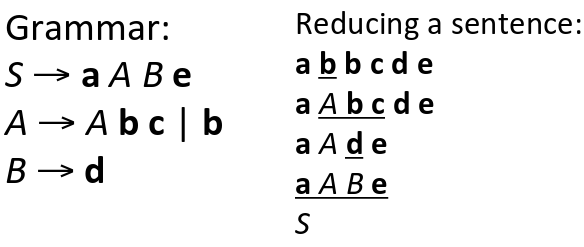
\includegraphics[scale=0.5]{res/image/shift_reduce}
\caption{Esempio \textit{Shift Reduce}}
\label{img:shift_reduce}
\end{center}
\end{figure}

Questa tecnica corrisponde alla \textit{rightmost derivation}. L'idea \`e
dalla stringa in input produrre l'albero di parsing partendo dalle foglie e
salire dai terminali fino ad arrivare al non-terminale iniziale.

\begin{figure}[H]
\begin{center}
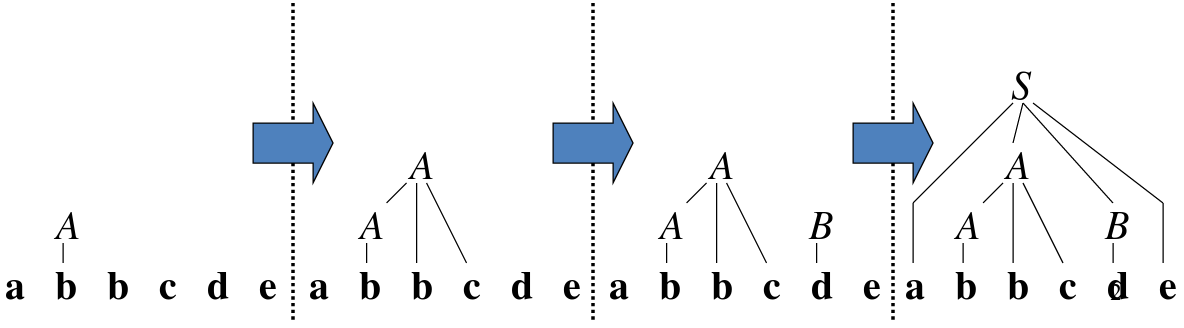
\includegraphics[scale=0.45]{res/image/shift_sequence}
\caption{Sequenza di passi della \textit{Shift Reduce}}
\label{img:shift_sequence}
\end{center}
\end{figure}

\subsubsection{Handles}
\begin{definition}[Handle]
Un handle in una forma sentenziale destra $\alpha$ \`e una produzione $A \to
\beta$ ed una posizione di $\beta$ in $\alpha$ tale che rimpiazzando $\beta$ con
$A$ noi otteniamo la precedente forma sentenziale destra nella derivazione
rightmost.
\end{definition}

Esempio:
\begin{figure}[H]
    \begin{subfigure}[b]{0.3\textwidth}
        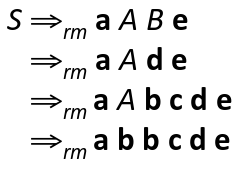
\includegraphics[scale=0.5]{res/image/rightmost}
        \caption{Derivazione \textit{rightmost}}
        \label{fig:rightmost}
    \end{subfigure}
    \quad
    \begin{subfigure}[b]{0.3\textwidth}
        \centering
        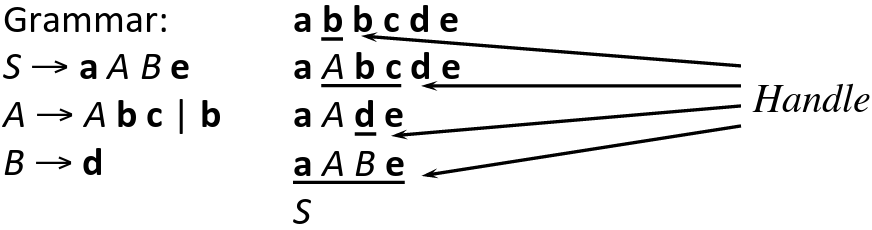
\includegraphics[scale=0.4]{res/image/handle}
        \caption{Insieme \textit{handle}}
        \label{fig:handle}
    \end{subfigure}
    \caption{Esempio \textit{handles}}
    \label{img:handles}
\end{figure}
prendiamo per il secondo \textit{handle}: $Abc$. Data grammatica in figura,
l'\textit{handle} \`e una produzione del non-terminale $A$ e come si pu\`o
vedere in fig.\ref{fig:rightmost} se si sotituisce alla sottostringa
\textit{handle} del quardo passo di derivazione con il non-terminale da dove
deriva si ottiene la forma sentenziale precedente ($a\mathbf{Abc}de \to
a\mathbf{A}de$).

\subsubsection{Implementazione Shift-Reduce Parsing}
Utilizzo di uno stack per effettuare le operazioni di riduzione. Lo stack e
l'input sono \textbf{sempre} nella forma sentenziale destra. Vi sono due
operazioni che si possono effettuare:
\begin{itemize}
\item \textbf{shift} - sposta il simbolo in input nel top dello stack
\item \textbf{reduce} - sostituisce, nella parte destra dello stack, i simboli
con il non-terminale da cui vengono prodotti
\end{itemize}

La \textit{reduce} avviene quando nel top dello stack \`e presento un
\textit{handle}. Quando si \`e arrivati al non-terminale di partenza nello stack
e l'input \`e vuoto allora il parsing si \`e concluso con successo.

\begin{figure}[H]
\begin{center}
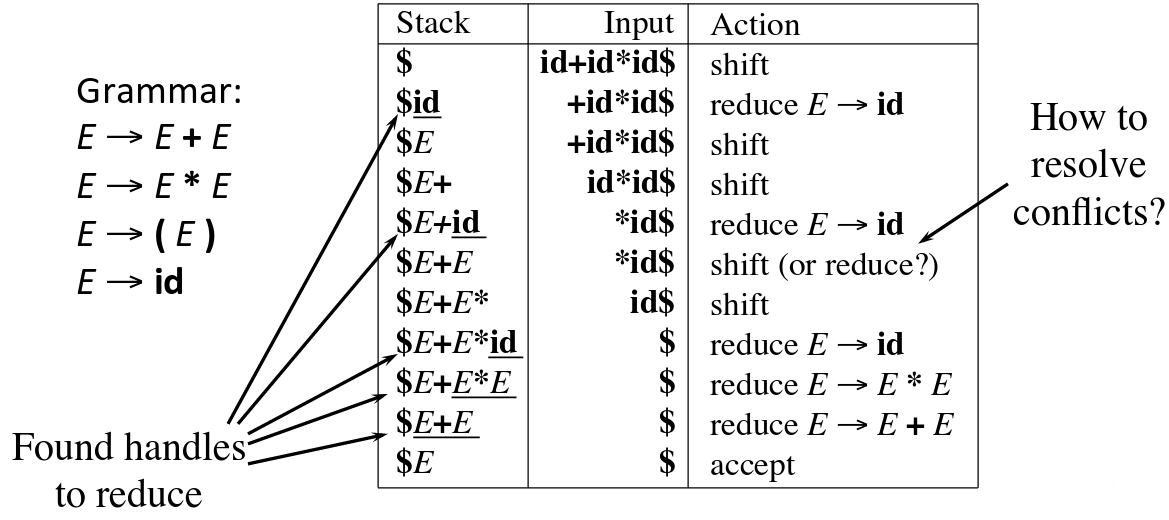
\includegraphics[scale=0.3]{res/image/shift_reduce_stack}
\caption{Esempio implementazione \textit{Shift Reduce}}
\label{img:shift_reduce_stack}
\end{center}
\end{figure}

\subsubsection{Risoluzione conflitti}
\label{sec:risoluzione_conflitti}
Come visto nella fig.\ref{img:shift_reduce_stack} vi \`e stato un caso in cui
non era chiaro se applicare uno \textit{shift} oppure la \textit{reduce}
($\$E+E \to_{shift} \$E+E^* \text{ oppure } \$E+E \to_{reduce} \$E$ ?). Questi
conflitti possono derivare dal \textbf{limite} del metodi di parsing $LR$ oppure
se la grammatica \`e ambigua (ma pu\`o anche non esserlo). Esistono due tipi
di conflitti:

\paragraph{Shift-Reduce}
esempio:
\begin{figure}[H]
\begin{center}
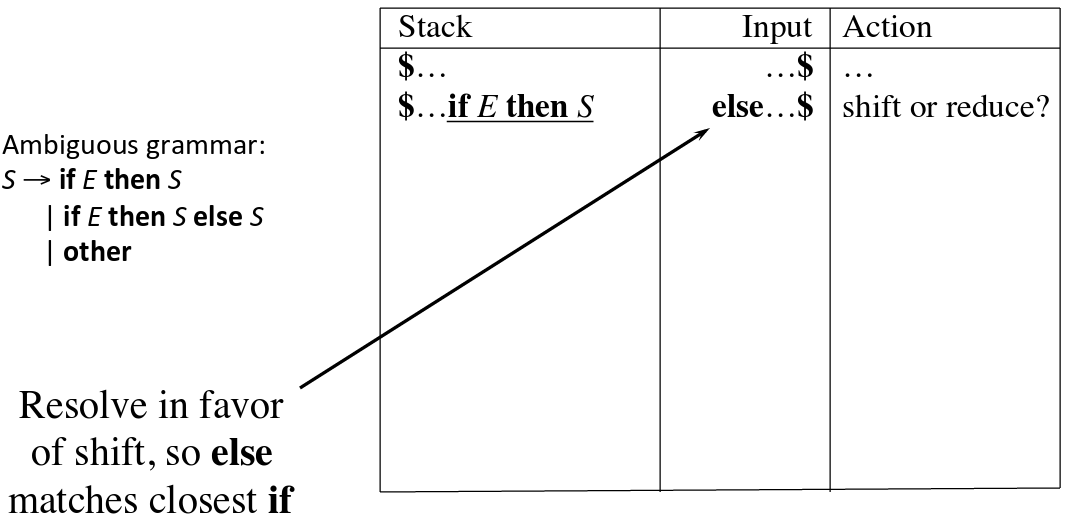
\includegraphics[scale=0.4]{res/image/shift-reduce}
\caption{Conflitto \textit{Shift-Reduce}}
\label{img:shift-reduce}
\end{center}
\end{figure}

\paragraph{Reduce-Reduce}
esempio:
\begin{figure}[H]
\begin{center}
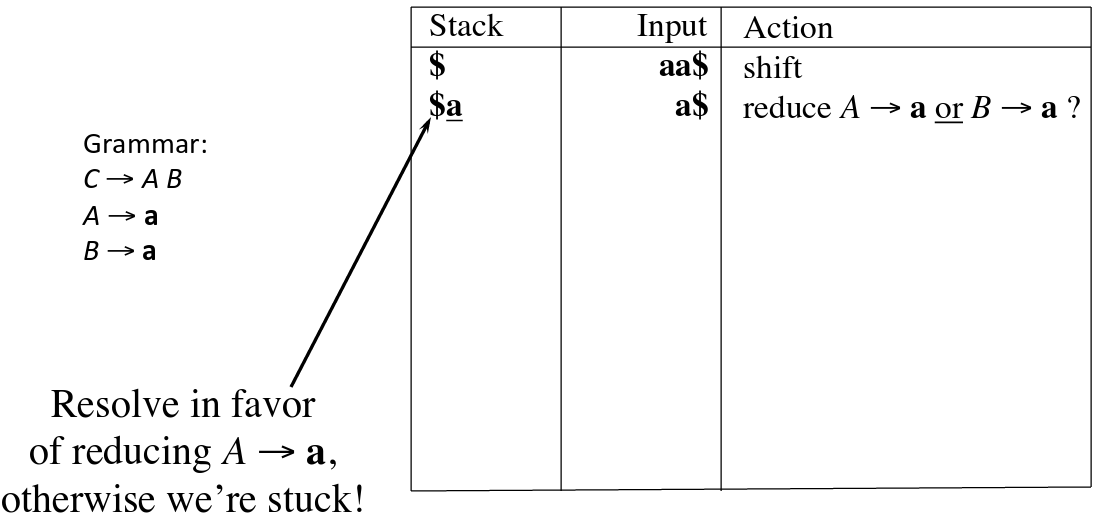
\includegraphics[scale=0.4]{res/image/reduce-reduce}
\caption{Conflitto \textit{Reduce-Reduce}}
\label{img:reduce-reduce}
\end{center}
\end{figure}

in entrambi i casi la soluzione addotta la costruzione di un DFA che rappresenti
gli \textbf{stati} della grammatica in base ai simboli consumanti. Il primo
stato (denominato $I_0$) contiene tutte le produzioni in cui \`e possibile
partire (dovrebbero essere tutte le produzioni dove appare il primo simbolo,
terminale e non possibile). Da qui si utilizza l'operatore $goto$ che
prendendo due parametri:
\begin{itemize}
\item stato di partenza $I_i \in I$
\item simbolo
\end{itemize}
restituisce lo stato successivo. Il DFA risultante potrebbe essere visto come un
albero nel quale le foglie determinano la soluzione ai conflitti
\textit{Shift-Reduce} o \textit{Reduce-Reduce}.

\begin{figure}[H]
\begin{center}
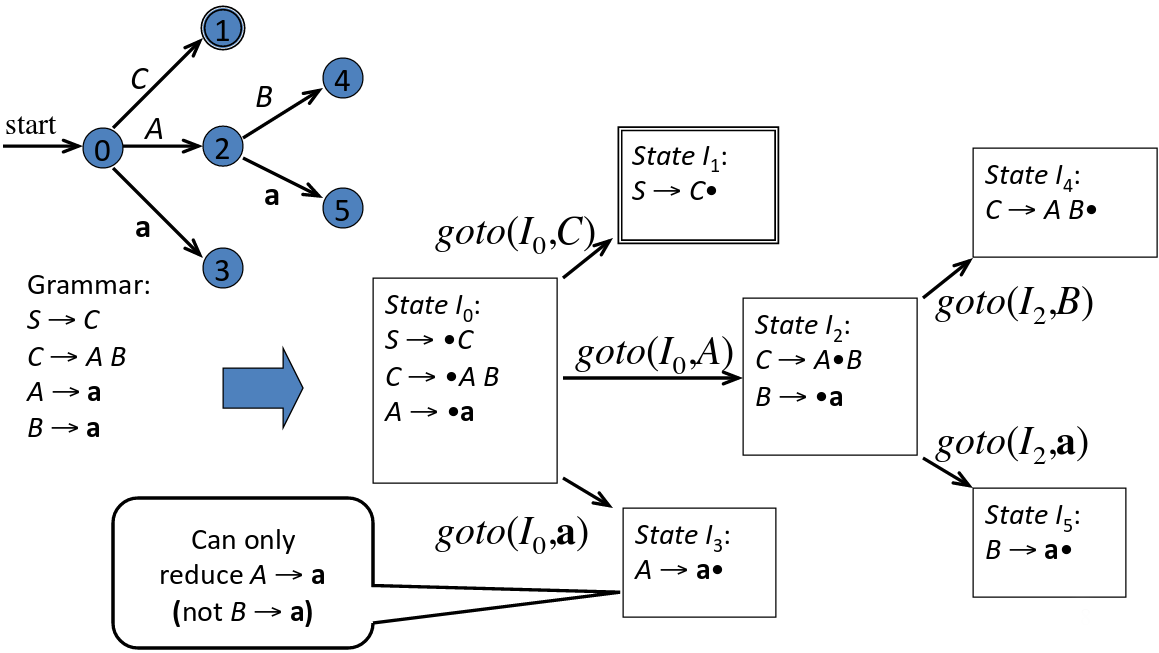
\includegraphics[scale=0.25]{res/image/dfa_shift_reduce}
\caption{DFA per soluzione conflitti}
\label{img:dfa_shift_reduce}
\end{center}
\end{figure}

\subsection{LR parser}
Il modello del parser $LR$ non discosta di molto da quello per $LL$ ma cambia
la tabella che pilota i comandi del \textit{driver}. Al posto delle produzione
da attuare in base al non-terminale ed al simbolo in input, ora si vanno a
descrivere due elementi:
\begin{itemize}
\item \textbf{actions} - l'azione da intraprendere (\textit{shift, reduce,
accept, error})
\item \textbf{goto} - la tabella rappresentante il DFA per la risoluzione dei
conflitti
\end{itemize}

\begin{figure}[H]
\centering
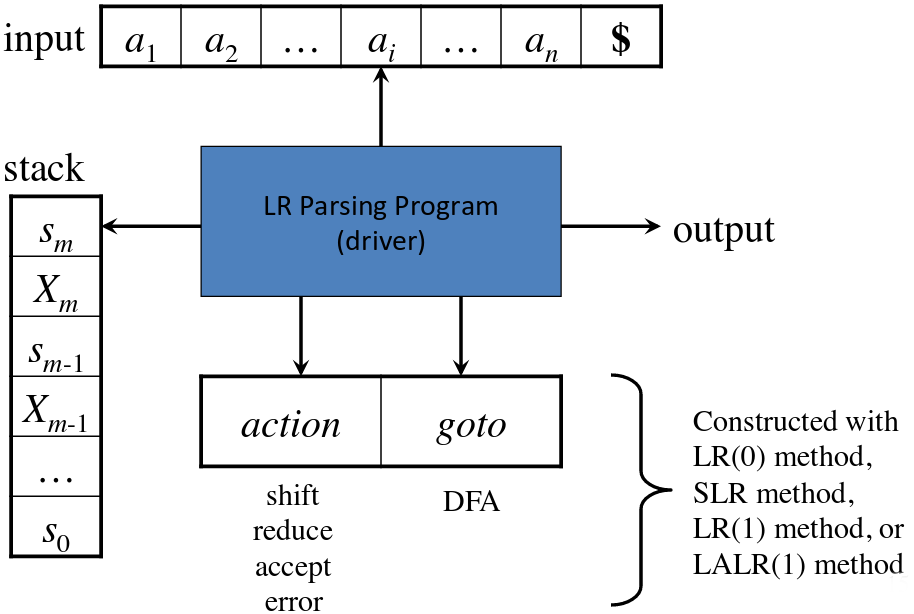
\includegraphics[scale=0.3]{res/image/LR_model}
\caption{Modello LR parser}
\label{img:LR_model}

\end{figure}
In base alle azioni descritta nella tabella \textit{action/goto} il driver
esegue le operazioni appropriate. Le azioni sono prese in base allo stato
attuale ($s_m$) e l'input attuale ($a_i$):

\paragraph{configuration (= LR parser state)}
$$(\underbrace{s_0X_1s_1X_2s_2...X_ms_m}_\text{stack},\
\underbrace{a_ia_{i+1}...a_n\$}_\text{input})$$

\paragraph{$\mathbf{action[s_m,a_i]=shift}$}
Dati i due input si inserisce nello stack il simbolo in input $a_i$ e lo stato
attuale $s$ nell'$LR$ automata.
$$(s_0X_1s_1X_2s_2...X_ms_ma_is,\ a_{i+1}...a_n\$)$$

\paragraph{$\mathbf{action[s_m,a_i]=reduce \ \alpha \to \beta}$}
Rimpiazzo nello stack tutta la forma sentenziale $\beta$ prodotta dal
non-terminale $A$ con direttamente $A$. Il DFS avanza nello stato $s$ indicato
nella tabella $goto[s_{m-r},A]$ dove $r=|\beta|$. Il valore dello stato sar\`a
inserito nel top dello stack.
$$(s_0X_1s_1X_2s_2...X_{m-r}s_{m-r}As,\ a_ia_{i+1}...a_n\$)$$

\paragraph{$\mathbf{action[s_m,a_i]=accept}$}
Parsing concluso.

\paragraph{$\mathbf{action[s_m,a_i]=error}$}
Attesa recupero. \\

Con $X_i$ indica il sibolo nella posizione $i$ dello stack. La tabella da cui il
driver prende decisioni sul parsing \`e creata a partire dall'automa a stati,
come in fig.\ref{img:from_DFA_to_table}. Se la produzione \textbf{iniziale}
contenesse produzioni \textbf{multiple} allora bisogna creare una produzione
aggiuntiva che la derivi (si noti $C'$).

\begin{figure}[H]
\centering
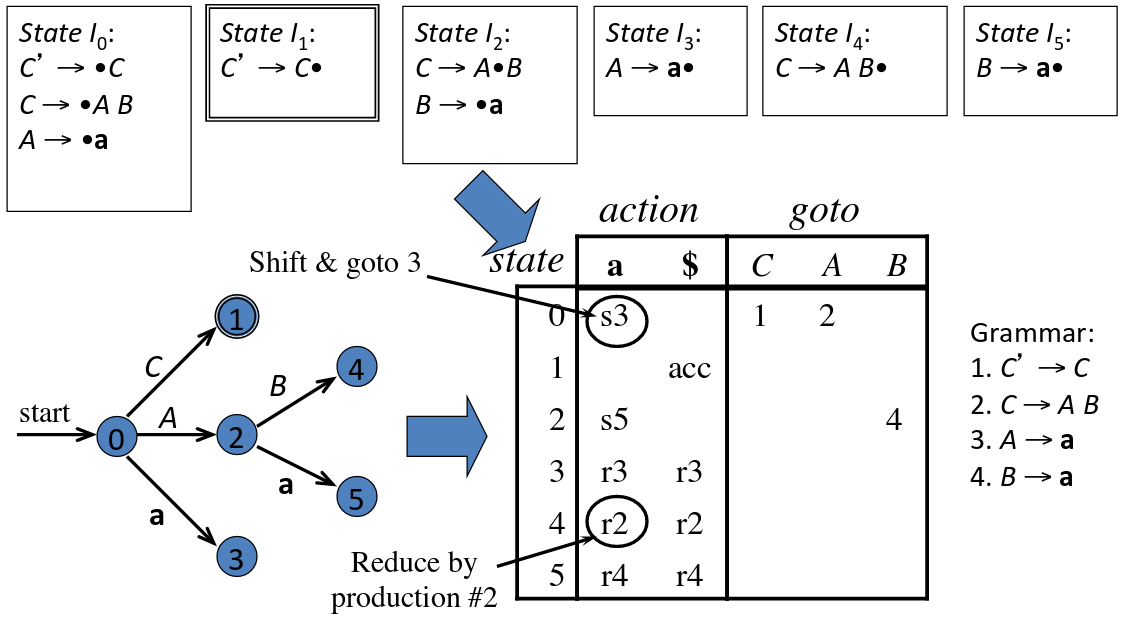
\includegraphics[scale=0.45]{res/image/from_DFA_to_table}
\caption{Esempio da $LR(0)$ automa all'$LR(0)$ tabella di parsing}
\label{img:from_DFA_to_table}
\end{figure}

\subsection{Verso l'automa LR(0)}
\subsubsection{LR(0) \textit{items} di una grammatica}
\begin{definition}[$LR(0)$ item]
Un $LR(0)$ item di una grammatica $G$ \`e una produzione di $G$ con un $\bullet$
in qualche posizione del lato destro.
\end{definition}

Intuitivamente si pu\`o considerare la posizione raggiunta durante il parsing.
Esempio: la produzione
$$A \to XYZ$$
ha quattro \textit{items}:
\begin{itemize}
\item $[A \to \bullet XYZ]$
\item $[A \to X \bullet YZ]$
\item $[A \to XY \bullet Z]$
\item $[A \to XYZ \bullet]$
\end{itemize}

Nel caso di $\epsilon$-produzioni della forma $A \to \epsilon$ c'\`e un unico
item: $[A \to \bullet]$.

\subsubsection{Viable prefix e valid items}
\label{sec:viable_prefix_and_valid_items}
\begin{definition}[Viable prefix]
Un viable prefix \`e un \textbf{prefisso} di una forma sentenziale destra che
non continua dopo la parte finale destra di un \textit{rightmost handle} di una
forma sentenziale.
\end{definition}

\begin{definition}[Valid item]
Un item $[A \to \beta_1 \bullet \beta_2]$ \`e valido per un viable prefix
$\alpha\beta_1$ se c'\`e una derivazione
$$S' \Rightarrow^*_{rm} \alpha Aw \Rightarrow_{rm} \alpha\beta_1\beta_2w $$
\end{definition}

Gli stati di un automa $LR(0)$ \`e l'insieme di item il quale sono
\textbf{validi per un viable prefix}.

\subsubsection{La chiusura per LR(0) item}
\begin{definition}[Closure operation for $LR(0)$ items]
Per un insieme di item $I$, definiamo $closure(I)$ come segue:
\begin{enumerate}
\item Parte con $closure(I) = I$
\item Se $[A \to \alpha\bullet B\beta] \in closure(I) \implies \forall B \to
\gamma$ della grammatica, aggiungi $[B \to \bullet\gamma]$ ad $I$ se non \`e
gi\`a presente
\item Ripetere 2 finch\'e nessun nuovo item pu\`o essere aggiunto
\end{enumerate}
\end{definition}

Da notare che se l'item $[A \to \alpha\bullet B\beta]$ \`e un
\textit{valid item} per un \textit{viable prefix} $\alpha_1\alpha$, allora anche
$[B \to \bullet\gamma]$ \`e valido per lui:
$$S' \Rightarrow^*_{rm} \alpha_1 Aw \Rightarrow_{rm} \alpha_1\alpha B\beta w
\Rightarrow_{rm} \alpha_1\alpha\gamma\beta w$$

\begin{figure}[H]
\centering
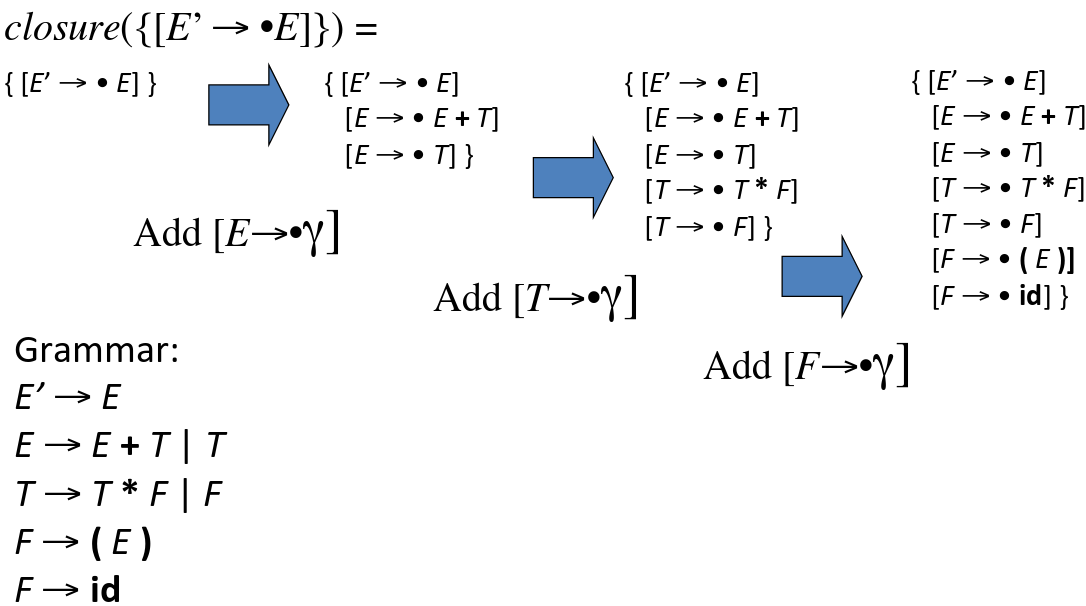
\includegraphics[scale=0.4]{res/image/closure_item}
\caption{Esempio $closure(I)$}
\label{img:closure_item}
\end{figure}

\subsubsection{Il goto per LR(0) item}
\begin{definition}[Goto operation for $LR(0)$ items]
Per un insieme di item $I$ e un simbolo $X$, si definisce $goto(I,X)$ come
segue:
\begin{enumerate}
\item $\forall [A \to \alpha \bullet X\beta] \in I$  aggiungi l'insieme
$closure(\{[A \to \alpha X \bullet\beta]\})$ ad $goto(I,X)$ se non \`e gi\`a
presente
\item ripetere 1 finch\'e non ci sono altri item da aggiungere a $goto(I,X)$
\end{enumerate}
\end{definition}

Intuitivamente, $goto(I,X)$ \`e l'insieme di item validi per il \textit{viable
prefix} $\gamma X$ quando $I$ \`e l'insieme di item che sono validi per
$\gamma$.

\begin{figure}[H]
\centering
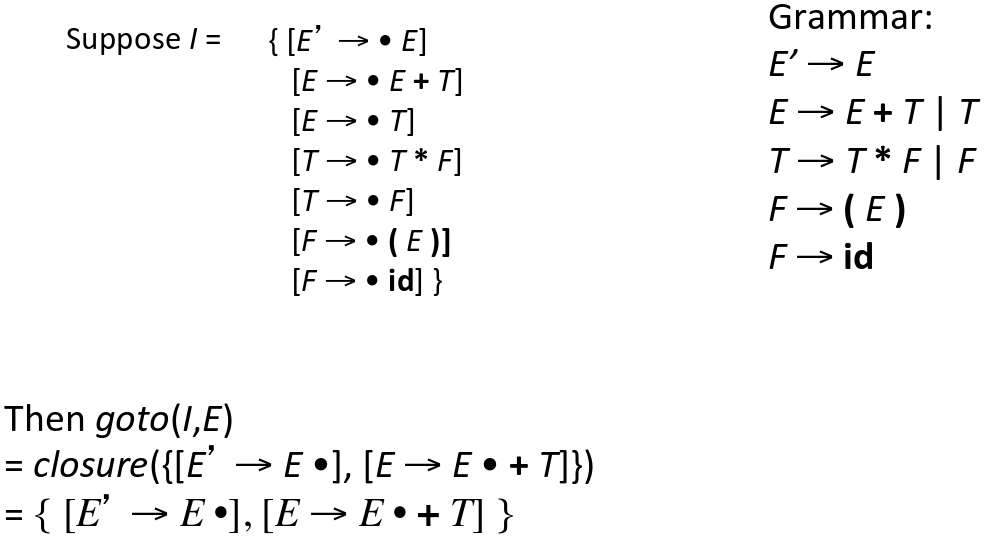
\includegraphics[scale=0.45]{res/image/goto_item}
\caption{Esempio $goto(I,X)$}
\label{img:goto_item}
\end{figure}

\subsubsection{Costruire l'insieme di LR(0) item di una grammatica}
\begin{enumerate}
\item La grammatica \`e aumentata con un \textbf{nuovo} simbolo iniziale $S'$ e
la produzione $S' \to S$
\item Inizialmente, insieme $C = closure(\{[S' \to \bullet S]\})$ (sar\`a lo
stato iniziale del DFA)
\item $\forall I \in C, \ X \in (N \cup T) \mid goto(I,X) \notin C \land
goto(I,X) \neq \emptyset$, aggiungere l'insieme di item $goto(I,X)$ in $C$
\item Ripetere 3 finch\'e non \`e pi\`u possibile aggiungere a $C$ insiemi di
item
\end{enumerate}

\begin{figure}[H]
\centering
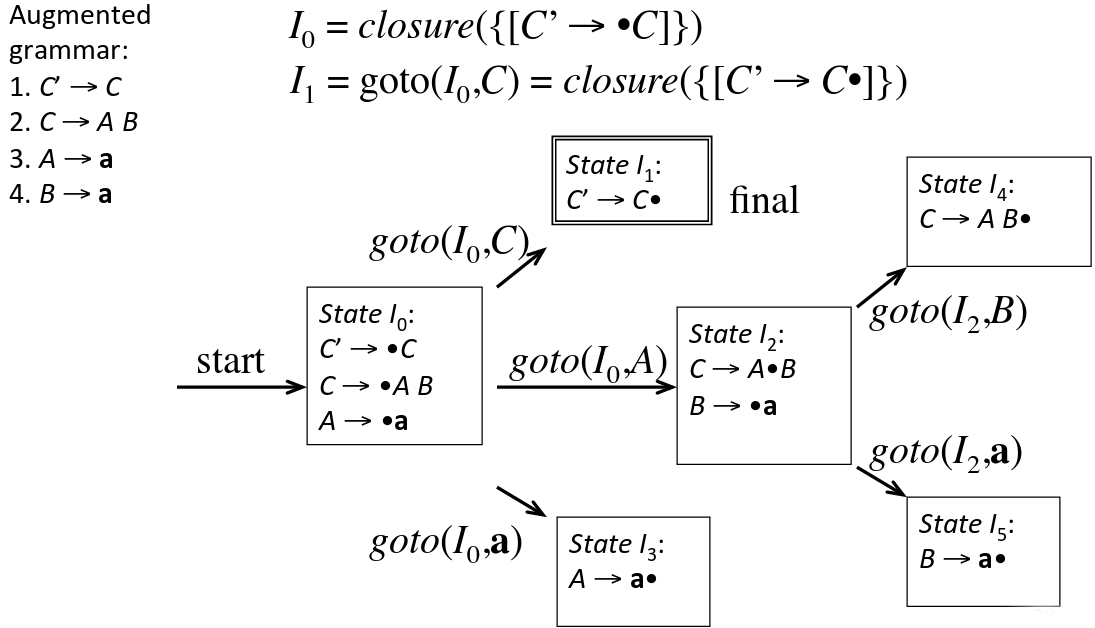
\includegraphics[scale=0.35]{res/image/LR_automaton}
\caption{Dalla grammatica all'automa $LR(0)$}
\label{img:LR_automaton}
\end{figure}

\subsection{SLR Parsing}
La costruzione della tabella per determinare le operazioni di
\textit{shift/reduce} avviene tramite usata dal parser $LR$ avviene utilizzando
l'$SLR$ \textit{parser}. Il parser parte dal DFA per la costruizione della
tabella utilizzando \textit{lookahead} per la risoluzione di eventuali
conflitti.

\begin{definition}[SLR]
SLR (Simple LR) \`e una semplice estensione del parsing $LR(0)$
\textit{shift-reduce}.
\end{definition}

L'$SLR$ elimina alcuni conflitti dalla popolazione della tabella di parsing con
riduzioni $A \to \alpha$ sui simboli in $FOLLOW(A)$.

\subsubsection{Passi costruzione della tabella di parsing}
\label{sec:step_parsing_table_construction_LR0}
\begin{enumerate}
\item Aumenta la grammatica con $S' \to S$
\item Costruire l'insieme $C = \{I_0,I_1,...,I_n\}$ di $LR(0)$ item
\item Se $[A \to \alpha\bullet a\beta] \in I_i \land goto(I_i,a)=I_j
\Rightarrow action[i,a] = \mathbf{shift} \ j$
\item Se $[A \to \alpha\bullet] \in I_i \Rightarrow action[i,a]=\mathbf{reduce}
\ A \to \alpha, \ \forall a \in FOLLOW(A)$ (applicare solo se $A \neq S'$)
\item Se $[S' \to S\bullet] \in I_i \Rightarrow action[i,\$] = \mathbf{accept}$
\item Se $goto(I_i,A)=I_j \Rightarrow goto[i,A]=j$
\item Ripetere da 3 a 6 finch\'e non ci sono pi\`u entry da aggiungere
\item Lo stato iniziale $i$ \`e lo $I_i$ item proprietario $[S' \to \bullet S]$
\end{enumerate}

Se vi sono \textbf{conflitti} nella costruzione della tabella allora la
grammatica \textbf{non \`e} $SLR$.

\begin{figure}[H]
\centering
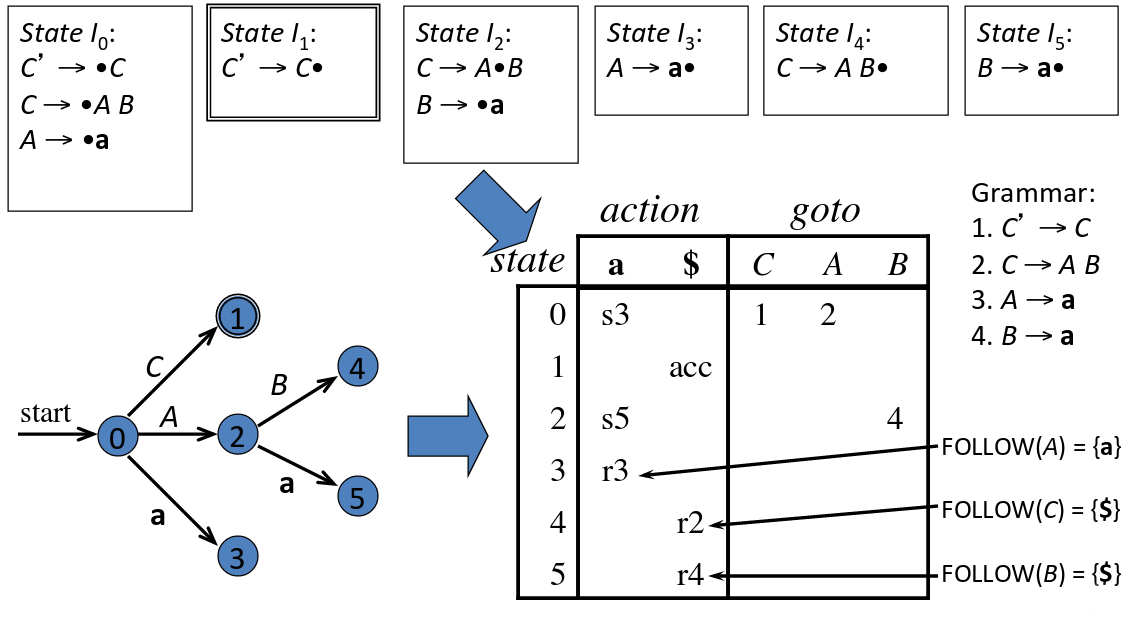
\includegraphics[scale=0.35]{res/image/LR_table}
\caption{Dall'automa $LR(0)$ alla tabella di parsing}
\label{img:LR_table}
\end{figure}

\subsubsection{SLR, ambiguit\`a e conflitti}
Le grammatiche $SLR$ sono tutte \textbf{non ambigue}, per\`o \textbf{non} tutte
le grammatiche non ambigue sono $SLR$. Come spiegato sopra, il motivo \`e l'
insorgere di conflitti durante la costruzione della tabella di parsing.

Esempio: Si consideri la grammatica
\begin{align*}
& S \to L=R & S \to R   \\
& L \to *R  & L \to id  \\
& R \to L
\end{align*}
\begin{figure}[H]
\centering
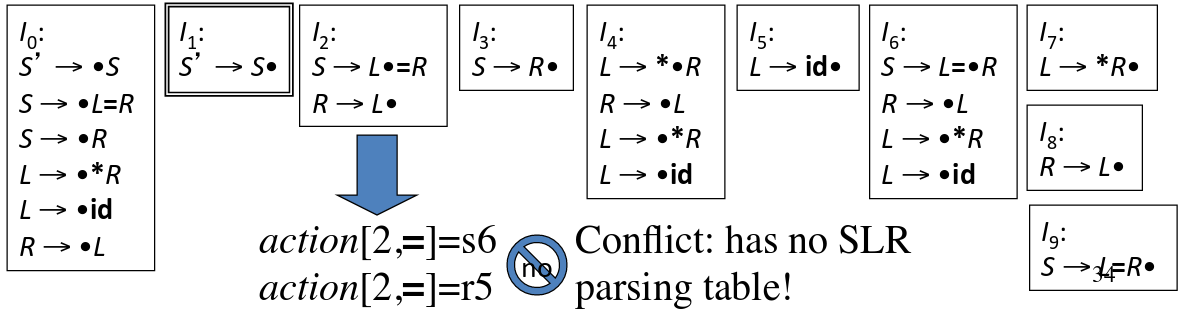
\includegraphics[scale=0.35]{res/image/SLR_table_conflict}
\caption{Grammatica non ambigua ma conflitti nella tabella $SLR$}
\label{img:SLR_table_conflict}
\end{figure}

\subsection{Grammatica LR(1)}
Le grammatiche $SLR$ sono troppo semplici, attraverso il parsing $LR(1)$ \`e
possibile evitare superflui conflitti nella tabella di parsing utilizzando un
\textit{lookahead}. Le grammatiche $LR(1)$ sono un super-insieme delle $LR(0)$
dove gli $LR(1) \ item = LR(0) \ item + lookahead$.
\begin{align*}
LR(0) &\ item: & LR(1) \ item: \\
[A \to& \alpha\bullet\beta]  & [A \to \alpha\bullet\beta, a]
\end{align*}

\subsubsection{Gli LR(1) item}
Gli item di $LR(1)$ riprendono quanto detto in $LR(0)$, tuttavia il loro
comportamento varia a seconda della forma della produzione all'interno dell'
item:

\paragraph{$\mathbf{[A \to \alpha\bullet\beta,a]}$}
Contengono un \textit{lookahead} terminale $a$, significa $\alpha$ gi\`a nel
top dello stack in attesa del parsing di $\beta a$. Inoltre con $\beta \neq
\epsilon$ il \textit{lookahead} non ha effetto.

\paragraph{$\mathbf{[A \to \alpha\bullet,a]}$}
Il \textit{lookahead} $a$ \`e usato per ridurre $A \to \alpha$ solo se il
possimo simbolo dell'input \`e $a$. Chiaramente $a \in FOLLOW(A)$, ma non tutti
i terminali dell'insieme appaiono come \textit{lookahead}.

\subsubsection{La chiusura per LR(1) item}
\begin{definition}[Closure operation for $LR(1)$ items]
Per un insieme di item $I$, definiamo $closure(I)$ come segue:
\begin{enumerate}
\item Parte con $closure(I) = I$
\item Se $[A \to \alpha\bullet B\beta,a] \in closure(I) \implies
\text{ aggiungi } [B \to \bullet\gamma, b]$ ad $I$ se non \`e gi\`a presente,
$\forall B \to \gamma \in P$ e $b \in FIRST(\beta a)$
\item Ripetere 2 finch\`e nessun nuovo item possa essere aggiunto
\end{enumerate}
\end{definition}

\subsubsection{Il goto per LR(1) item}
\begin{definition}[Goto operation for $LR(1)$ items]
Per un insieme di item $I$ ed un simbolo $X$, si definisce $goto(I,X)$ come
segue:
\begin{enumerate}
\item $\forall [A \to \alpha\bullet X\beta,a] \in I$ aggiungi l'insieme di item
$closure(\{[A \to \alpha X\bullet\beta,a]\})$ a $goto(I,X)$ se non \`e gi\`a
presente
\item Ripetere 1 finch\`e nessun'altro item pu\`o essere aggiunto a $goto(I,X)$
\end{enumerate}
\end{definition}

\subsubsection{Costuire l'insieme LR(1) di item di una grammatica}
\begin{enumerate}
\item Aumentare la grammatica con un nuovo simbolo iniziale $S'$ e la produzione
$S' \to S$
\item Inizialmente, insieme $C = closure(\{[S' \to \bullet S, \$]\})$ (questo
\`e lo stato iniziale del DFA)
\item $\forall I \in C, \ X \in (N \cup T) \mid goto(I,X) \notin C \land
goto(I,X) \neq \emptyset$, aggiungi l'insieme $goto(I,X)$ a $C$
\item Ripetere 4 finch\`e nessun'altro item pu\`o essere aggiunto a $C$
\end{enumerate}

\subsubsection{Costruzione \textit{Canonical LR(1) Parsing Tables}}
\label{sec:step_parsing_table_construction_LR1}
\begin{enumerate}
\item Aumento della grammatica con $S' \to S$
\item Costruire l'insieme $C = \{I_1,I_2,...,I_n\}$ di $LR(1)$ item
\item Se $[A \to \alpha\bullet a\beta,b] \in I_i \land goto(I_i,X)=I_j
\Rightarrow action[i,a]=\mathbf{shift} \ j$
\item Se $[A \to \alpha\bullet, a] \in I_i \Rightarrow action[i,a]=
\mathbf{reduce} \ A \to \alpha$ (applicare solo se $A \neq S'$)
\item Se $[S' \to S\bullet, \$] \in I_i \Rightarrow action[i,\$]=
\mathbf{accept}$
\item Se $goto(I_i,A)=I_j \Rightarrow goto[i,A]=j$
\item Ripetere ad 3 a 6 finch\`e nessun'altra entry sono aggiunte
\item Lo stato iniziale $i$ \`e lo $I_i$ proprietario di $[S' \to \bullet S,
\$]$
\end{enumerate}

\subsubsection{Esempio da grammatica a tabella}
\begin{figure}[H]
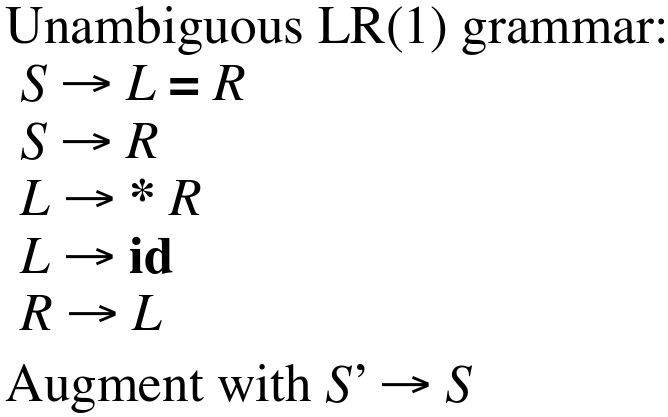
\includegraphics[scale=0.3]{res/image/ex_grammar}
\caption{Definizione grammatica ed aumento}
\label{fig:ex_grammar}
\end{figure}

\begin{figure}[H]
\centering
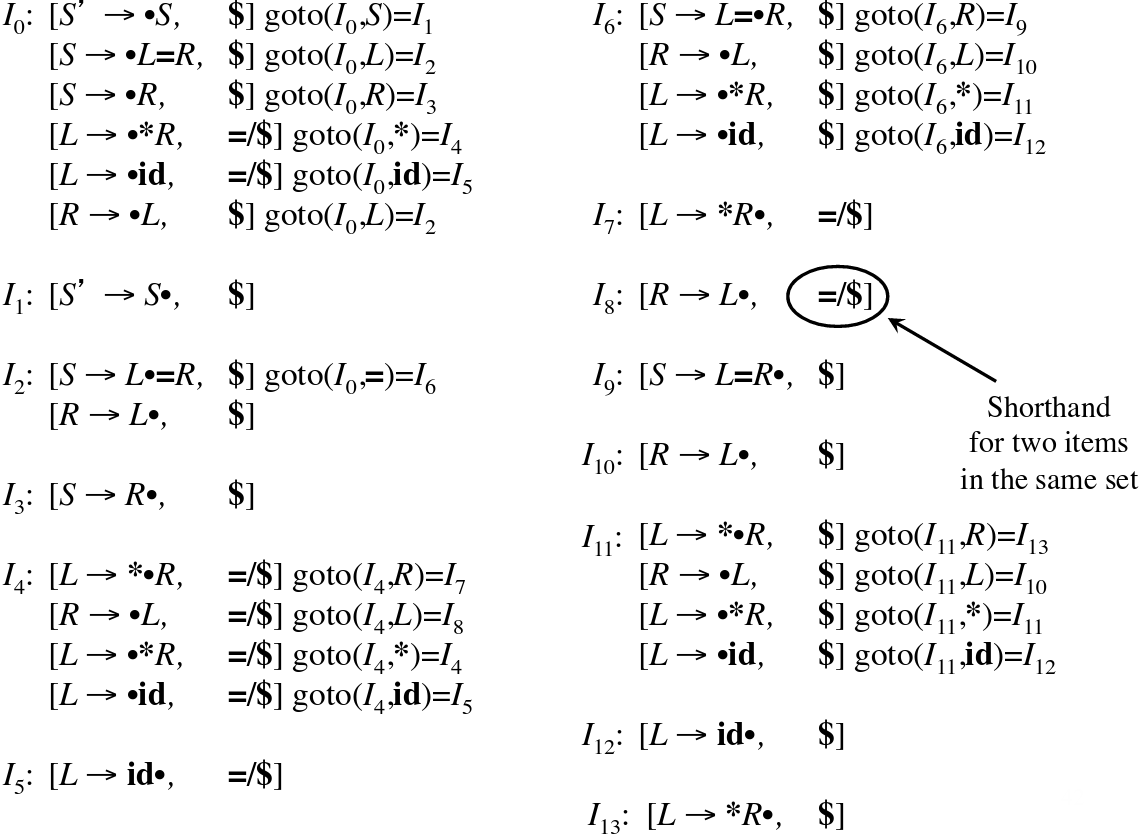
\includegraphics[scale=0.35]{res/image/ex_DFA}
\caption{Formulazione $LR(1)$ item della grammatica aumentata}
\label{fig:ex_DFA}
\end{figure}

\begin{figure}[H]
\centering
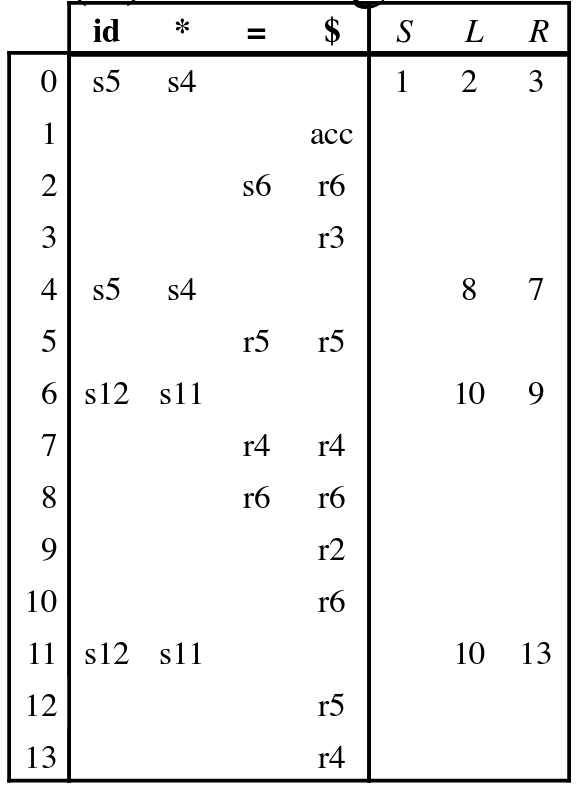
\includegraphics[scale=0.45]{res/image/ex_table}
\caption{Formulazione tabella di parsing della grammatica aumentata}
\label{fig:ex_table}
\end{figure}

\subsection{Parsing LALR}
\label{sec:parse_lalr}
Un difetto del parsign $LR(1)$ \`e che la sua tabella ha molti stati. Attraverso
il $LARL$ parsing si vuole effettuare un \textbf{merge} tra due o pi\`u stati
$LR(1)$ per ridurre le dimensioni della tabella. Tuttiavia $LARL$ \`e meno
potente di $LR(1)$:
\begin{itemize}
\item non saranno introdotti conflitti \textit{shift-reduce}, perch\'e lo
$shift$ non utilizza il \textit{lookahead}
\item potrebbero introdursi conflitti \textit{reduce-reduce}, ma di
\textbf{rado} succedono per grammatiche di linguaggi di programmazione
\end{itemize}

La costruzione della tabella $LARL$ \`e preceduta dalla formulazione del DFA
$LR(1)$ canonica. Una volta conclusa si esegue il merge tra insieme di item che
\textbf{condividono la stessa prima parte}.

\begin{figure}[H]
\centering
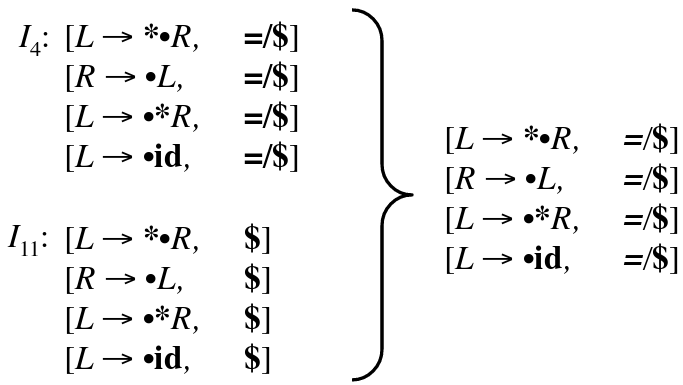
\includegraphics[scale=0.5]{res/image/share_LALR}
\caption{Merge degli item}
\label{fig:share_LALR}
\end{figure}

\subsection{Considerazioni generali}
Una grammatica \`e $X$ se la sua tabella di parsing $X$ \textbf{non ha}
conflitti. $X$ \`e:
\begin{itemize}
\item $LL(1)$ o
\item $SLR$ o
\item $LR(1)$ o
\item $LALR$
\end{itemize}

La relazione tra i linguaggi supportati dai parsing visti:
\begin{figure}[H]
\centering
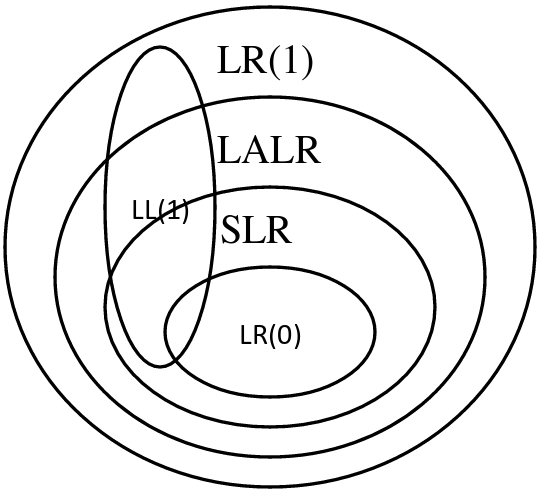
\includegraphics[scale=0.5]{res/image/relation_parser}
\caption{Relazione linguaggi dei parser}
\label{fig:relation_parser}
\end{figure}
